\documentclass[11pt]{article}

% ---------------------- Packages ----------------------
\usepackage[margin=1in]{geometry}
\usepackage[T1]{fontenc}
\usepackage[utf8]{inputenc}
\usepackage{lmodern}
\usepackage{microtype}
\usepackage{amsmath,amssymb,mathtools}
\usepackage{booktabs,array,tabularx,longtable}
\usepackage[table]{xcolor}
\usepackage{enumitem}
\usepackage{tikz}
\usetikzlibrary{arrows.meta,positioning,fit,calc,shapes.geometric,decorations.pathreplacing,backgrounds,matrix}
\usepackage{pgfplots}
\pgfplotsset{compat=1.18}
\tikzset{every node/.append style={align=center}}
\usepackage[most]{tcolorbox}
\usepackage{hyperref}
\usepackage{bookmark}
\usepackage{fancyhdr}
\usepackage{lastpage}
\usepackage{caption}
\usepackage{float}
\usepackage{multicol}
\usepackage{needspace}

% ---------------------- Colors and style ----------------------
\definecolor{deepblue}{HTML}{1F4E79}
\definecolor{softblue}{HTML}{D9EAF7}
\definecolor{softgreen}{HTML}{DFF1DF}
\definecolor{softorange}{HTML}{FCE4D6}
\definecolor{softpurple}{HTML}{E8DDF4}
\definecolor{softgray}{HTML}{F2F2F2}
\definecolor{darkgreen}{HTML}{2E6B3E}
\definecolor{darkorange}{HTML}{C65911}
\definecolor{darkpurple}{HTML}{6B3FA0}
\definecolor{darkred}{HTML}{8B1E1E}
\definecolor{lightyellow}{HTML}{FFF2CC}

\hypersetup{
  colorlinks=true,
  linkcolor=deepblue,
  urlcolor=deepblue,
  citecolor=deepblue,
  pdftitle={A High-School Friendly Tutorial on the Cell2location Bayesian Model},
  pdfauthor={OpenAI},
  pdfsubject={Bayesian inference and spatial transcriptomics},
  pdfkeywords={Bayesian inference, cell2location, spatial transcriptomics, negative binomial, hyperparameters}
}

\pagestyle{fancy}
\fancyhf{}
\lhead{Cell2location Bayesian model tutorial}
\rhead{\thepage}
\renewcommand{\headrulewidth}{0.4pt}
\setlength{\headheight}{14pt}

\setlength{\parskip}{0.65em}
\setlength{\parindent}{0pt}
\setlist[itemize]{topsep=0.3em,itemsep=0.2em,leftmargin=1.5em}
\setlist[enumerate]{topsep=0.3em,itemsep=0.2em,leftmargin=1.7em}
\renewcommand{\arraystretch}{1.25}

\newcommand{\dd}{\mathrm{d}}
\newcommand{\NB}{\mathrm{NB}}
\newcommand{\Pois}{\mathrm{Pois}}
\newcommand{\E}{\mathbb{E}}
\newcommand{\Var}{\mathrm{Var}}
\newcommand{\Data}{\text{data}}
\newcommand{\Unknowns}{\text{unknowns}}
\newcommand{\spot}{\text{spot}}
\newcommand{\gene}{\text{gene}}
\newcommand{\celltype}{\text{cell type}}
\newcommand{\mRNA}{\text{mRNA}}
\newcommand{\scRNA}{\text{single-cell RNA-seq}}

\newtcolorbox{bigidea}{
  breakable,
  colback=softblue,
  colframe=deepblue,
  boxrule=0.8pt,
  arc=2mm,
  left=1mm,right=1mm,top=1mm,bottom=1mm,
  title=Big idea,
  fonttitle=\bfseries
}

\newtcolorbox{warningbox}{
  breakable,
  colback=softorange,
  colframe=darkorange,
  boxrule=0.8pt,
  arc=2mm,
  left=1mm,right=1mm,top=1mm,bottom=1mm,
  title=Common confusion,
  fonttitle=\bfseries
}

\newtcolorbox{mathbox}{
  breakable,
  colback=softgray,
  colframe=black!50,
  boxrule=0.6pt,
  arc=2mm,
  left=1.5mm,right=1.5mm,top=1.5mm,bottom=1.5mm,
  title=Model piece,
  fonttitle=\bfseries
}

\newtcolorbox{checkpoint}{
  breakable,
  colback=softgreen,
  colframe=darkgreen,
  boxrule=0.8pt,
  arc=2mm,
  left=1mm,right=1mm,top=1mm,bottom=1mm,
  title=Check your understanding,
  fonttitle=\bfseries
}

\newtcolorbox{assumptionbox}{
  breakable,
  colback=lightyellow,
  colframe=darkred,
  boxrule=0.7pt,
  arc=2mm,
  left=1mm,right=1mm,top=1mm,bottom=1mm,
  title=Assumption,
  fonttitle=\bfseries
}

\newcommand{\term}[1]{\textbf{#1}}
\newcommand{\code}[1]{\texttt{#1}}

% ---------------------- Document ----------------------
\begin{document}

\begin{titlepage}
\centering
\vspace*{0.5in}
{\Huge\bfseries A High-School Friendly Tutorial\\[0.3em]
On the Cell2location Bayesian Model\par}
\vspace{0.35in}
{\Large Explaining the model shown on page 12 of\\
\emph{Cell2location maps fine-grained cell types in spatial transcriptomics}\par}
\vspace{0.55in}
\begin{tcolorbox}[colback=softblue,colframe=deepblue,width=0.88\textwidth,arc=2mm]
\large
This tutorial explains the page-12 Bayesian model step by step: what is observed, what is unknown, what is being modeled, what the symbols mean, why priors are used, and why the two user-adjusted hyperparameters matter.
\end{tcolorbox}
\vfill
{\large Prepared as a learning guide for a high school student}\par
\vspace{0.3in}
{\large \today}\par
\end{titlepage}

\tableofcontents
\newpage

\section{What problem is cell2location trying to solve?}

Imagine a thin slice of tissue, such as a slice of mouse brain or a human lymph node. A spatial transcriptomics machine measures many small locations on the tissue. In a common technology such as 10x Visium, each location, often called a \term{spot}, can contain RNA from more than one cell.

For each spot, the machine gives a table of counts:

\begin{center}
\begin{tabular}{c|cccc}
\toprule
Spot & Gene 1 & Gene 2 & Gene 3 & Gene 4 \\
\midrule
Spot A & 18 & 0 & 43 & 6 \\
Spot B & 2 & 31 & 7 & 20 \\
Spot C & 15 & 12 & 10 & 4 \\
\bottomrule
\end{tabular}
\end{center}

These counts are not direct labels like ``this spot has 3 T cells and 1 B cell.'' They are just gene-expression counts. The job of cell2location is to use those gene counts to estimate:

\begin{center}
\fbox{\Large How much of each cell type is present at each spot?}
\end{center}

\begin{bigidea}
Cell2location is a Bayesian model for turning gene counts at tissue locations into estimated cell-type abundances. It uses reference cell-type signatures from single-cell or single-nucleus RNA-seq, then asks: ``Which mixture of reference cell types most likely produced the observed gene counts at this spot?''
\end{bigidea}

\subsection{Why do we need a model at all?}

If every spot contained exactly one cell, and every cell type had one perfect marker gene, the problem would be easy. But real data are messy:

\begin{itemize}
  \item A spot may contain several cells.
  \item Different cell types can express many of the same genes.
  \item Some cell types are very similar to each other.
  \item The machine may capture more RNA in some spots than in others.
  \item Some RNA floating around in the experiment may contaminate a spot.
  \item Counts are noisy. Repeating the same experiment would not give exactly the same numbers.
\end{itemize}

A model is a careful mathematical story for how the observed counts could have been generated. Bayesian inference then runs this story backward: from observed counts to likely hidden cell-type abundances.

\begin{figure}[H]
\centering
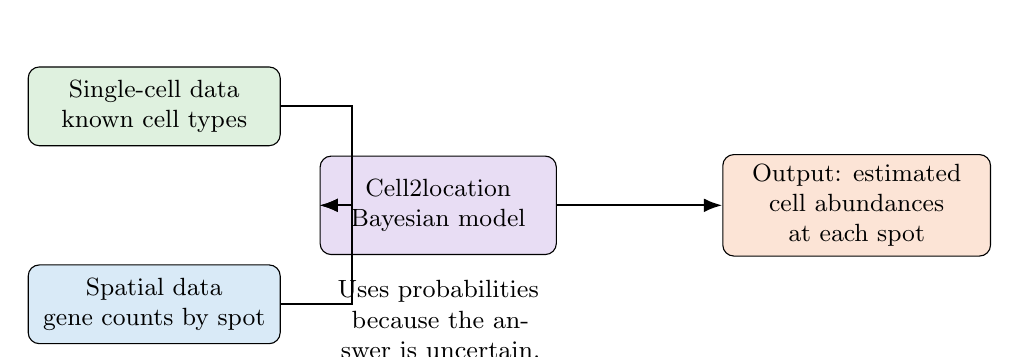
\begin{tikzpicture}[node distance=1.5cm, every node/.style={font=\small,align=center}, >=Latex]
  \node[draw, rounded corners, fill=softgreen, minimum width=3.2cm, minimum height=1.0cm] (single) {Single-cell data\\known cell types};
  \node[draw, rounded corners, fill=softblue, below=of single, minimum width=3.2cm, minimum height=1.0cm] (spatial) {Spatial data\\gene counts by spot};
  \node[draw, rounded corners, fill=softpurple, right=2.1cm of $(single)!0.5!(spatial)$, minimum width=3.0cm, minimum height=1.25cm] (model) {Cell2location\\Bayesian model};
  \node[draw, rounded corners, fill=softorange, right=2.1cm of model, minimum width=3.4cm, minimum height=1.25cm] (out) {Output: estimated\\cell abundances\\at each spot};
  \draw[->, thick] (single.east) -- ++(0.9,0) |- (model.west);
  \draw[->, thick] (spatial.east) -- ++(0.9,0) |- (model.west);
  \draw[->, thick] (model) -- (out);
  \node[align=center, below=0.2cm of model, text width=3.7cm] {Uses probabilities because the answer is uncertain.};
\end{tikzpicture}
\caption{A simplified workflow. Single-cell data tell us what each cell type usually expresses. Spatial data tell us what was observed at each spot. Cell2location combines them.}
\end{figure}

\section{A tiny biology and data dictionary}

You do not need to be a biologist to understand the model, but these words help.

\begin{longtable}{>{\bfseries}p{0.22\textwidth}p{0.70\textwidth}}
\toprule
Term & Plain-English meaning \\
\midrule
Gene & A DNA instruction. In this model, we only care about how much RNA from a gene is detected. \\
\mRNA & Messenger RNA. More mRNA from a gene usually means that gene is more active. \\
RNA count & The number reported by the sequencing technology for a gene in a spot. Counts are nonnegative whole numbers: 0, 1, 2, and so on. \\
Cell type & A category of cell, such as T cell, B cell, astrocyte, or neuron subtype. \\
Reference signature & A typical gene-expression pattern for one cell type. It says things like: ``T cells usually have high expression of gene A and low expression of gene B.'' \\
Spatial spot/location & A small location on the tissue slide. It may contain several cells or parts of cells. \\
Batch/experiment & A slide, sample, or technology run. Two batches can have different technical behavior. \\
\bottomrule
\end{longtable}

\newpage
\section{Bayesian inference in one page}

The whole Bayesian idea can be written as:

\begin{mathbox}
\[
\underbrace{p(\Unknowns \mid \Data)}_{\text{posterior}}
\;\propto\;
\underbrace{p(\Data \mid \Unknowns)}_{\text{likelihood}}
\times
\underbrace{p(\Unknowns)}_{\text{prior}}.
\]
\end{mathbox}

Read it like this:

\begin{itemize}
  \item \term{Unknowns}: things we want to learn, such as how many cells of each type are in each spot.
  \item \term{Data}: the gene counts we observed.
  \item \term{Likelihood}: how well a possible answer explains the data.
  \item \term{Prior}: what the model thinks is reasonable before looking at this particular spot's data.
  \item \term{Posterior}: the updated beliefs after seeing the data.
\end{itemize}

\begin{bigidea}
Bayesian inference is not just one best answer. It is a way to describe uncertainty. Instead of only saying ``there are 4 B cells,'' it can say ``the abundance is probably around 4, but values around 3 or 5 are also possible.''
\end{bigidea}

\subsection{A non-biological analogy: guessing candies in a jar}

Suppose you cannot see inside a jar, but you can hear a few clues when the jar shakes. You want to guess how many red, blue, and green candies are inside.

\begin{itemize}
  \item The hidden numbers of candies are the \term{unknowns}.
  \item The sounds you hear are the \term{data}.
  \item Your belief that the jar probably has 20-50 candies, not 10,000, is a \term{prior}.
  \item A physical model connecting candies to sounds is the \term{likelihood}.
  \item Your final best guesses after hearing the sounds are the \term{posterior}.
\end{itemize}

Cell2location is similar, except the ``jar'' is a tissue spot, the ``candy colors'' are cell types, and the ``sounds'' are RNA counts from genes.

\section{Which things have a model?}

This is one of the most important points.

\begin{warningbox}
Students often ask: ``Which one should have a model? The data? The parameters? The prior?'' The answer is: a Bayesian model has a probability model for the observed data \emph{given} unknown quantities, and probability models called priors for unknown quantities. You do not put a prior on the observed numbers after you have observed them; they are fixed data. You put priors on unknowns.
\end{warningbox}

For cell2location, a helpful classification is:

\begin{longtable}{p{0.25\textwidth}p{0.22\textwidth}p{0.45\textwidth}}
\toprule
Thing & Role & Explanation \\
\midrule
Observed spatial count $d_{s,g}$ & Data & The measured RNA count of gene $g$ at spot $s$. This is what the model tries to explain. \\
Reference signature $g_{f,g}$ & Input to mapping step & Typical expression of gene $g$ for cell type $f$. Page 12 treats this as an input when mapping cell types to spots. It is usually estimated from single-cell data first. \\
Cell abundance $w_{s,f}$ & Main unknown & How much cell type $f$ is present at spot $s$. This is the main answer we want. \\
Expected count $\mu_{s,g}$ & Hidden expected value & The model's predicted average count for gene $g$ at spot $s$. \\
Technical factors $m_g$, $s_{e,g}$, $y_s$ & Unknown adjustment parameters & These help explain technology differences, background RNA, and spot-by-spot RNA capture. \\
Overdispersion $\alpha_{e,g}$ & Noise parameter & Controls how noisy the count distribution is for gene $g$ in experiment $e$. \\
Hyperparameters $\hat N$, $\alpha^y$ & User-set prior knobs & These control priors: expected cells per spot and how much spot sensitivity can vary. \\
\bottomrule
\end{longtable}

\begin{bigidea}
The main unknown is $w_{s,f}$: the abundance of cell type $f$ at spot $s$. Most of the model exists to estimate $w_{s,f}$ while not being fooled by noisy counts and technical effects.
\end{bigidea}


\section{Bayes' rule for the actual cell2location formula}
\label{sec:bayes-rule-cell2location}

This section answers a very common question: in the general formula

\[
p(\theta\mid \Data)=\frac{p(\Data\mid \theta)p(\theta)}{p(\Data)},
\]

what is \(\theta\) for cell2location?

\begin{bigidea}
Your instinct is right: the most important part of \(\theta\) is \(w_{s,f}\), the abundance of cell type \(f\) at spot \(s\). But the full model has other unknown parameters too, such as \(m_g\), \(y_s\), \(s_{e,g}\), and \(\alpha_{e,g}\). These are not the main biological answer, but the model needs them so that technical effects do not get mistaken for cell-type abundance.
\end{bigidea}

\subsection{First split the unknowns into two groups}

It is helpful to separate the unknowns into the main unknowns and the helper unknowns.

\begin{mathbox}
\[
\underbrace{W=\{w_{s,f}\}}_{\text{main biological unknowns}}
\qquad
\underbrace{\Phi=\{m_g,\,y_s,\,s_{e,g},\,\alpha_{e,g}\}}_{\text{helper / technical unknowns}}.
\]
\end{mathbox}

Here \(W\) is a big table. One row is a spatial spot, and one column is a cell type.
For example, \(w_{17,\mathrm{astrocyte}}\) means ``estimated astrocyte abundance in spot 17.''

The symbol \(\Phi\) is just a convenient name for all the other unknowns. These other unknowns are sometimes called \term{nuisance parameters}. That name does \emph{not} mean they are useless. It means they are not the final scientific answer we mainly care about, but we must still estimate or account for them.

\subsection{The full Bayes' rule version}

Let

\begin{itemize}
  \item \(D=\{d_{s,g}\}\) be the observed spatial gene-count data.
  \item \(\Gamma=\{g_{f,g}\}\) be the reference cell-type signatures from single-cell data.
  \item \(H\) be the hyperparameters, such as \(\hat N\), \(\alpha^y\), and the chosen number \(R\) of shared tissue patterns.
\end{itemize}

Then the full Bayesian formula can be written as:

\begin{mathbox}
\[
\boxed{
p(W,\Phi \mid D,\Gamma,H)
=
\frac{
\overbrace{p(D\mid W,\Phi,\Gamma)}^{\text{likelihood}}
\;\overbrace{p(W,\Phi\mid H)}^{\text{prior}}
}{
\underbrace{p(D\mid \Gamma,H)}_{\text{evidence / normalizing denominator}}
}
}
\]
\end{mathbox}

This is the same Bayes' rule as before, but with names that match cell2location.

\subsection{What is on the numerator?}

The numerator is the important part to understand:

\begin{mathbox}
\[
\begin{aligned}
\text{numerator}
&= \text{likelihood}\times\text{prior} \\
&= p(D\mid W,\Phi,\Gamma)\times p(W,\Phi\mid H).
\end{aligned}
\]

The likelihood asks: ``How well does this proposed explanation predict the observed counts?''
The prior asks: ``How reasonable was this proposed explanation before seeing these counts?''
\end{mathbox}

Now plug in the negative binomial observation model:

\begin{mathbox}
\[
\boxed{
p(D\mid W,\Phi,\Gamma)
=
\prod_{s=1}^{S}\prod_{g=1}^{G}
\NB\!\left(
 d_{s,g}\;\middle|\;
 \mu_{s,g},\alpha_{e(s),g}
\right)
}
\]
\[
\boxed{
\mu_{s,g}
=
\left(
 m_g\sum_{f=1}^{F}w_{s,f}g_{f,g}+s_{e(s),g}
\right)y_s.
}
\]
\end{mathbox}

The notation \(e(s)\) means ``the experiment or batch that spot \(s\) belongs to.'' If there is only one experiment, you can ignore this detail.

The prior part can be shown conceptually like this:

\begin{mathbox}
\[
p(W,\Phi\mid H)
=
\underbrace{p(W\mid \hat N,R,\ldots)}_{\text{prior for cell abundances}}
\underbrace{p(Y\mid \alpha^y,\ldots)}_{\text{prior for spot sensitivities}}
\underbrace{p(M)p(B)p(A)}_{\text{priors for other technical/noise parameters}}.
\]
\end{mathbox}

In that last line, \(Y=\{y_s\}\), \(M=\{m_g\}\), \(B=\{s_{e,g}\}\), and \(A=\{\alpha_{e,g}\}\). The page-12 Methods text does not list every prior distribution in the main article; it points to the Supplementary Methods for the complete derivation. For a beginner, the key idea is that the numerator is always:

\[
\text{likelihood} \times \text{prior}.
\]

\subsection{What is the denominator doing?}

The denominator is

\begin{mathbox}
\[
p(D\mid \Gamma,H)
=
\int p(D\mid W,\Phi,\Gamma)p(W,\Phi\mid H)\,\dd W\,\dd\Phi.
\]
\end{mathbox}

This means: add up the numerator over all possible values of the unknowns. Its job is to make the posterior probabilities add up to 1. In many huge models, this integral is too hard to calculate exactly, which is why cell2location uses approximate variational inference.

\begin{warningbox}
The denominator is not a new biological assumption. It is a normalizing constant. In practice, many explanations of Bayes' rule use \(\propto\), meaning ``proportional to,'' because the numerator is what compares one possible explanation against another.
\end{warningbox}

\subsection{If we only care about \texorpdfstring{$w_{s,f}$}{w_sf}}

Usually, the final answer we want is \(W=\{w_{s,f}\}\): the cell-type abundance map. But because \(m_g\), \(y_s\), \(s_{e,g}\), and \(\alpha_{e,g}\) are also unknown, a careful Bayesian answer averages over them:

\begin{mathbox}
\[
p(W\mid D,\Gamma,H)
=
\int p(W,\Phi\mid D,\Gamma,H)\,\dd\Phi.
\]
\end{mathbox}

In words:

\begin{quote}
To learn the cell abundances \(W\), consider all plausible technical settings \(\Phi\), and average over their uncertainty.
\end{quote}

So if a previous simple tutorial wrote \(\theta\), you can read it in two ways:

\begin{itemize}
  \item \term{Simple version:} \(\theta=W\), the cell abundance table.
  \item \term{Full version:} \(\theta=(W,\Phi)\), all unknown quantities in the model.
\end{itemize}

\subsection{A tiny numerical example}

Suppose one spot has two possible cell types: neurons and astrocytes. For one gene, the reference signatures are:

\[
g_{\mathrm{neuron},g}=2,
\qquad
 g_{\mathrm{astrocyte},g}=20.
\]

Now imagine the model is testing this possible explanation:

\[
w_{s,\mathrm{neuron}}=3,
\qquad
w_{s,\mathrm{astrocyte}}=4,
\qquad
m_g=0.5,
\qquad
s_{e,g}=1,
\qquad
y_s=1.2.
\]

Then the expected count is

\[
\begin{aligned}
\mu_{s,g}
&=\left(m_g\sum_f w_{s,f}g_{f,g}+s_{e,g}\right)y_s \\
&=\left(0.5\bigl(3\cdot 2+4\cdot 20\bigr)+1\right)1.2 \\
&=\left(0.5(86)+1\right)1.2 \\
&=52.8.
\end{aligned}
\]

If the observed count was \(d_{s,g}=50\), this proposed explanation would get a fairly good likelihood for this gene because 50 is close to 52.8. If the observed count was \(d_{s,g}=5\), this proposed explanation would get a much worse likelihood for this gene.

\begin{figure}[H]
\centering
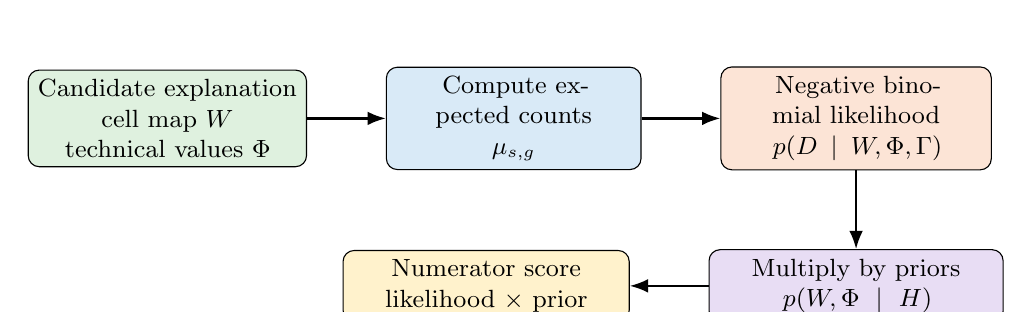
\begin{tikzpicture}[node distance=1.1cm, every node/.style={font=\small,align=center}, >=Latex]
  \node[draw, rounded corners, fill=softgreen, text width=3.3cm] (candidate) {Candidate explanation\\cell map \(W\)\\technical values \(\Phi\)};
  \node[draw, rounded corners, fill=softblue, right=1.0cm of candidate, text width=3.0cm] (mu) {Compute expected counts\\\(\mu_{s,g}\)};
  \node[draw, rounded corners, fill=softorange, right=1.0cm of mu, text width=3.2cm] (like) {Negative binomial likelihood\\\(p(D\mid W,\Phi,\Gamma)\)};
  \node[draw, rounded corners, fill=softpurple, below=1.0cm of like, text width=3.5cm] (prior) {Multiply by priors\\\(p(W,\Phi\mid H)\)};
  \node[draw, rounded corners, fill=lightyellow, left=1.0cm of prior, text width=3.4cm] (num) {Numerator score\\likelihood \(\times\) prior};
  \draw[->, thick] (candidate) -- (mu);
  \draw[->, thick] (mu) -- (like);
  \draw[->, thick] (like) -- (prior);
  \draw[->, thick] (prior) -- (num);
\end{tikzpicture}
\caption{The numerator of Bayes' rule gives a score to each possible explanation. Good explanations both predict the observed counts well and satisfy the prior assumptions.}
\end{figure}

\subsection{Parameter or hyperparameter?}

Here is the classification in the page-12 formula.

\begin{longtable}{>{\raggedright\arraybackslash}p{0.12\textwidth}>{\raggedright\arraybackslash}p{0.30\textwidth}>{\raggedright\arraybackslash}p{0.18\textwidth}>{\raggedright\arraybackslash}p{0.32\textwidth}}
\toprule
Symbol & Plain-English meaning & Role & Learned or chosen? \\
\midrule
\(d_{s,g}\) & Observed count of gene \(g\) at spot \(s\) & Data & Observed, not learned \\
\(g_{f,g}\) & Reference expression of gene \(g\) in cell type \(f\) & Input to spatial model & Estimated earlier from single-cell data, then treated as fixed input for mapping \\
\(w_{s,f}\) & Abundance of cell type \(f\) at spot \(s\) & Main parameter & Learned from the spatial data \\
\(\mu_{s,g}\) & Expected count for gene \(g\) at spot \(s\) & Deterministic hidden mean & Computed from the parameters, not usually a separate free parameter \\
\(m_g\) & Gene-specific technology sensitivity multiplier & Parameter & Learned; helps adjust differences between technologies \\
\(s_{e,g}\) & Gene- and experiment-specific additive background shift & Parameter & Learned; helps account for contaminating/background RNA \\
\(y_s\) & Spot-specific RNA detection sensitivity & Parameter & Learned; its prior is controlled by \(\alpha^y\) \\
\(\alpha_{e,g}\) & Gene- and experiment-specific overdispersion/noise & Parameter & Learned or estimated as part of the model's noise behavior \\
\(\hat N\) & Expected number of cells per spot & Hyperparameter & Chosen by the user, often using histology images \\
\(\alpha^y\) & Strength of regularization for \(y_s\) & Hyperparameter & Chosen by the user; large values keep \(y_s\) closer to the batch average \\
\(R\) & Number of shared abundance patterns in the hierarchical prior & Model setting & Chosen before fitting; the paper usually sets \(R=50\) \\
\bottomrule
\end{longtable}

\begin{checkpoint}
A quick test: is \(y_s\) a hyperparameter because it has a prior? No. \(y_s\) is a parameter. The hyperparameter is \(\alpha^y\), because \(\alpha^y\) controls the prior over \(y_s\).
\end{checkpoint}


\section{The page-12 model, rewritten gently}

Page 12 describes the cell2location model in compact mathematical notation. Here is the main model in a beginner-friendly form.

\subsection{Step 1: the observed counts are noisy counts}

\begin{mathbox}
\[
\boxed{d_{s,g} \sim \NB(\mu_{s,g},\alpha_{e,g})}
\]
\end{mathbox}

This says:

\begin{quote}
The observed count $d_{s,g}$ for spot $s$ and gene $g$ is treated as a random count drawn from a negative binomial distribution with average level $\mu_{s,g}$ and noise/overdispersion $\alpha_{e,g}$.
\end{quote}

Breakdown:

\begin{itemize}
  \item $s$ means a spatial spot or location.
  \item $g$ means a gene.
  \item $e$ means the experiment or batch containing that spot.
  \item $d_{s,g}$ is observed. Example: spot 17 has 42 counts of gene \code{ACTB}.
  \item $\mu_{s,g}$ is the model's expected average count.
  \item $\alpha_{e,g}$ lets the count be more variable than a simple Poisson count.
\end{itemize}

\subsection{Why negative binomial?}

Counts are whole numbers. A simple count model is the Poisson distribution, but real RNA counts are usually more variable than Poisson. The negative binomial distribution is a common way to model count data with extra variability.

\begin{figure}[H]
\centering
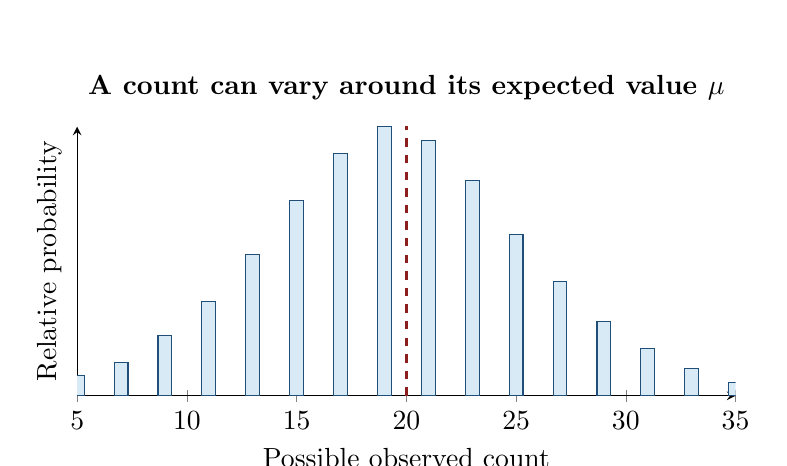
\begin{tikzpicture}
\begin{axis}[
  width=0.82\textwidth,
  height=5cm,
  xlabel={Possible observed count},
  ylabel={Relative probability},
  ymin=0,
  xtick={5,10,15,20,25,30,35},
  ytick=\empty,
  axis lines=left,
  title={A count can vary around its expected value $\mu$},
  title style={font=\bfseries},
  bar width=5pt
]
\addplot[ybar, fill=softblue, draw=deepblue] coordinates {
(5,0.03) (7,0.05) (9,0.09) (11,0.14) (13,0.21) (15,0.29) (17,0.36)
(19,0.40) (21,0.38) (23,0.32) (25,0.24) (27,0.17) (29,0.11) (31,0.07) (33,0.04) (35,0.02)
};
\draw[darkred, very thick, dashed] (axis cs:20,0) -- (axis cs:20,0.43);
\node[darkred, anchor=south] at (axis cs:20,0.43) {$\mu$};
\end{axis}
\end{tikzpicture}
\caption{A schematic count distribution. Even if the expected count is about $20$, the observed count might be $17$, $22$, or another nearby value. The negative binomial distribution allows more spread than the simplest count model.}
\end{figure}

\begin{checkpoint}
If a model predicts $\mu_{s,g}=20$, does it require the observed count to be exactly $20$? No. It says counts near 20 are more plausible than counts very far away, but random variation is allowed.
\end{checkpoint}

\newpage
\subsection{Step 2: expected gene counts are built from cell-type mixtures}

The model defines $\mu_{s,g}$ like this:

\begin{mathbox}
\[
\boxed{
\mu_{s,g}
=
\left(
\underbrace{m_g}_{\substack{\text{gene/technology}\\\text{sensitivity}}}
\underbrace{\sum_{f=1}^{F} w_{s,f}g_{f,g}}_{\substack{\text{cell-type}\\\text{contributions}}}
+
\underbrace{s_{e,g}}_{\substack{\text{background}\\\text{RNA shift}}}
\right)
\underbrace{y_s}_{\substack{\text{spot-level}\\\text{sensitivity}}}
}
\]
\end{mathbox}

This formula is the heart of the model. It says:

\begin{quote}
The expected RNA count for a gene at a spot equals the sum of contributions from all possible cell types, corrected for technology, background RNA, and the spot's RNA-capture sensitivity.
\end{quote}

\subsection{The most important part: the sum over cell types}

Focus first on this part:

\[
\sum_{f=1}^{F} w_{s,f}g_{f,g}.
\]

Here:

\begin{itemize}
  \item $F$ is the number of reference cell types.
  \item $f$ is one cell type, such as T cell, B cell, astrocyte subtype, neuron subtype, and so on.
  \item $g_{f,g}$ is the reference signature: how much gene $g$ is expected in one unit of cell type $f$.
  \item $w_{s,f}$ is the estimated amount of cell type $f$ at spot $s$.
\end{itemize}

\begin{bigidea}
The sum is a weighted recipe. Each cell type has a gene-expression recipe. The weights $w_{s,f}$ say how much of each recipe to mix into spot $s$.
\end{bigidea}

\begin{figure}[H]
\centering
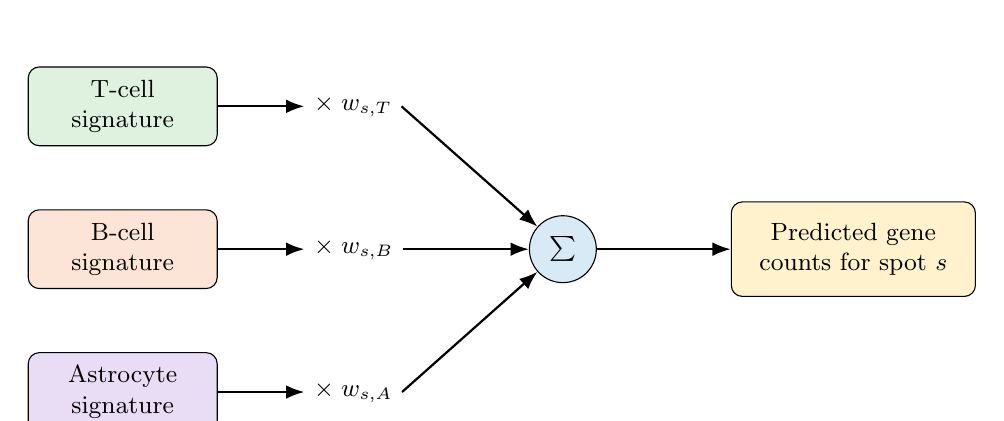
\begin{tikzpicture}[every node/.style={font=\small,align=center}, >=Latex]
  \node[draw, rounded corners, fill=softgreen, minimum width=2.4cm, minimum height=1.0cm] (t) {T-cell\\signature};
  \node[draw, rounded corners, fill=softorange, below=0.8cm of t, minimum width=2.4cm, minimum height=1.0cm] (b) {B-cell\\signature};
  \node[draw, rounded corners, fill=softpurple, below=0.8cm of b, minimum width=2.4cm, minimum height=1.0cm] (a) {Astrocyte\\signature};

  \node[right=1.1cm of t] (wt) {$\times\; w_{s,T}$};
  \node[right=1.1cm of b] (wb) {$\times\; w_{s,B}$};
  \node[right=1.1cm of a] (wa) {$\times\; w_{s,A}$};

  \node[draw, circle, fill=softblue, minimum size=0.85cm, right=1.6cm of wb] (sum) {$\sum$};
  \node[draw, rounded corners, fill=lightyellow, right=1.7cm of sum, minimum width=3.1cm, minimum height=1.2cm] (out) {Predicted gene\\counts for spot $s$};

  \draw[->, thick] (t.east) -- (wt.west);
  \draw[->, thick] (b.east) -- (wb.west);
  \draw[->, thick] (a.east) -- (wa.west);
  \draw[->, thick] (wt.east) -- (sum);
  \draw[->, thick] (wb.east) -- (sum);
  \draw[->, thick] (wa.east) -- (sum);
  \draw[->, thick] (sum) -- (out);
\end{tikzpicture}
\caption{Each reference signature is multiplied by its abundance in the spot, then the contributions are added. This is why the model is called a decomposition model: it decomposes a mixed spot into cell-type pieces.}
\end{figure}

\section{A worked example with small numbers}

Let us use only two cell types and three genes. This is much smaller than real data, but it shows the idea.

\subsection{Reference signatures}

Suppose single-cell data tell us the typical gene counts per cell type look like this:

\begin{center}
\begin{tabular}{lccc}
\toprule
Reference signature & Gene A & Gene B & Gene C \\
\midrule
T cell & 8 & 0 & 4 \\
B cell & 0 & 7 & 3 \\
\bottomrule
\end{tabular}
\end{center}

Interpretation:

\begin{itemize}
  \item Gene A is high in T cells and low in B cells.
  \item Gene B is high in B cells and low in T cells.
  \item Gene C is expressed by both.
\end{itemize}

Now suppose one spatial spot has observed counts:

\begin{center}
\begin{tabular}{lccc}
\toprule
Observed spot & Gene A & Gene B & Gene C \\
\midrule
Spot $s$ & 15 & 25 & 16 \\
\bottomrule
\end{tabular}
\end{center}

\subsection{Try a possible answer}

Maybe spot $s$ contains about 2 T cells and 3 B cells. That means:

\[
w_{s,T}=2,
\qquad
w_{s,B}=3.
\]

Then the expected contributions are:

\begin{center}
\begin{tabular}{lccc}
\toprule
Contribution & Gene A & Gene B & Gene C \\
\midrule
$2$ T cells & $2\cdot 8=16$ & $2\cdot 0=0$ & $2\cdot 4=8$ \\
$3$ B cells & $3\cdot 0=0$ & $3\cdot 7=21$ & $3\cdot 3=9$ \\
\midrule
Predicted total $\mu$ & 16 & 21 & 17 \\
Observed count $d$ & 15 & 25 & 16 \\
\bottomrule
\end{tabular}
\end{center}

This is not perfect, but it is close. Because the count model is noisy, close can still be very likely.

\subsection{Try a bad answer}

If the spot had 0 T cells and 5 B cells, then Gene A would be predicted near 0, but the observed Gene A count is 15. So that answer is less plausible.

\begin{center}
\begin{tabular}{lccc}
\toprule
Candidate mixture & Predicted Gene A & Predicted Gene B & Good explanation? \\
\midrule
$2$ T cells, $3$ B cells & 16 & 21 & Reasonably good \\
$0$ T cells, $5$ B cells & 0 & 35 & Bad for Gene A \\
$5$ T cells, $0$ B cells & 40 & 0 & Bad for Gene B \\
\bottomrule
\end{tabular}
\end{center}

\begin{bigidea}
The likelihood gives higher probability to mixtures whose predicted counts are close to the observed counts, while still allowing noise.
\end{bigidea}

\section{Now add the technical correction terms}

The simple mixture $\sum_f w_{s,f}g_{f,g}$ is not enough for real data. Page 12 adds three correction terms:

\[
\mu_{s,g}=\left(m_g\sum_f w_{s,f}g_{f,g}+s_{e,g}\right)y_s.
\]

\subsection{The gene/technology sensitivity term $m_g$}

$m_g$ adjusts for gene-specific differences between technologies or datasets. Maybe the reference signatures came from one type of RNA-seq, but the spatial data came from another. Some genes may appear systematically higher or lower in one technology.

\begin{center}
\begin{tabularx}{0.95\textwidth}{>{\bfseries}p{0.18\textwidth}X}
\toprule
Symbol & Meaning \\
\midrule
$m_g$ & A gene-specific multiplier. It says whether gene $g$ tends to be detected more or less strongly in the spatial technology compared with the reference. \\
\bottomrule
\end{tabularx}
\end{center}

If $m_g=2$, then the model doubles the contribution of gene $g$ before comparing to spatial counts. If $m_g=0.5$, it halves it.

\subsection{The additive background term $s_{e,g}$}

$s_{e,g}$ allows for extra RNA not explained by cells in the spot. In experiments, a little RNA can float around or contaminate a region. This background can depend on the experiment $e$ and gene $g$.

\begin{center}
\begin{tabularx}{0.95\textwidth}{>{\bfseries}p{0.18\textwidth}X}
\toprule
Symbol & Meaning \\
\midrule
$s_{e,g}$ & A gene- and experiment-specific additive shift. It can explain background or contaminating RNA. \\
\bottomrule
\end{tabularx}
\end{center}

Important: $s_{e,g}$ is \emph{added}. The model says, roughly, ``Even before considering spot-specific capture sensitivity, maybe this experiment has some extra background for this gene.''

\subsection{The spot sensitivity term $y_s$}

$y_s$ is a multiplier for a whole spot. Some spots capture more RNA than others because of tissue quality, chemistry, or technical differences.

\begin{center}
\begin{tabularx}{0.95\textwidth}{>{\bfseries}p{0.18\textwidth}X}
\toprule
Symbol & Meaning \\
\midrule
$y_s$ & A spot-specific multiplier. If spot $s$ captures twice as much RNA, $y_s$ might be larger; if it captures less RNA, $y_s$ might be smaller. \\
\bottomrule
\end{tabularx}
\end{center}

\begin{figure}[H]
\centering
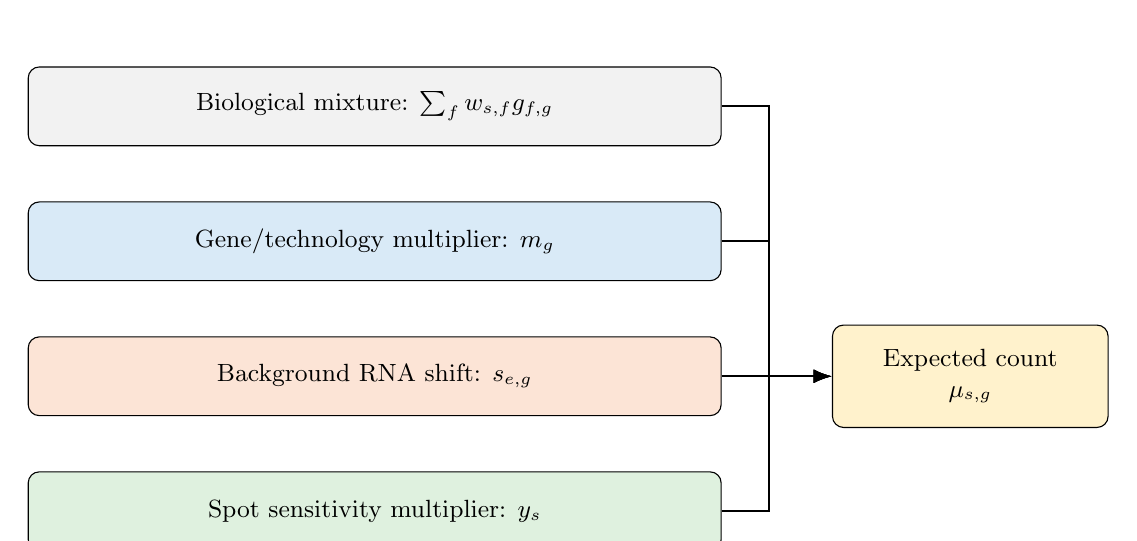
\begin{tikzpicture}[every node/.style={font=\small,align=center}, >=Latex]
  \node[draw, rounded corners, fill=softgray, minimum width=8.8cm, minimum height=1.0cm] (mix) {Biological mixture: $\sum_f w_{s,f}g_{f,g}$};
  \node[draw, rounded corners, fill=softblue, below=0.7cm of mix, minimum width=8.8cm, minimum height=1.0cm] (mg) {Gene/technology multiplier: $m_g$};
  \node[draw, rounded corners, fill=softorange, below=0.7cm of mg, minimum width=8.8cm, minimum height=1.0cm] (bg) {Background RNA shift: $s_{e,g}$};
  \node[draw, rounded corners, fill=softgreen, below=0.7cm of bg, minimum width=8.8cm, minimum height=1.0cm] (ys) {Spot sensitivity multiplier: $y_s$};
  \node[draw, rounded corners, fill=lightyellow, right=1.4cm of bg, minimum width=3.5cm, minimum height=1.3cm] (mu) {Expected count\\$\mu_{s,g}$};
  \draw[->, thick] (mix.east) -- ++(0.6,0) |- (mu.west);
  \draw[->, thick] (mg.east) -- ++(0.6,0) |- (mu.west);
  \draw[->, thick] (bg.east) -- (mu.west);
  \draw[->, thick] (ys.east) -- ++(0.6,0) |- (mu.west);
\end{tikzpicture}
\caption{The expected count $\mu_{s,g}$ is not only biology. It also includes technical adjustments.}
\end{figure}

\begin{warningbox}
Without $y_s$, a spot with low RNA capture might look like it has fewer cells. Without $m_g$, technology differences can look like biological differences. Without $s_{e,g}$, background RNA can be mistaken for a cell type. These correction terms help the model avoid those mistakes.
\end{warningbox}

\section{What exactly is $w_{s,f}$?}

The symbol $w_{s,f}$ is the star of the model.

\begin{mathbox}
\[
w_{s,f} = \text{estimated abundance of cell type } f \text{ at spot } s.
\]
\end{mathbox}

If $w_{s,B}=3.2$, the model is saying that spot $s$ contains an amount of B-cell RNA roughly comparable to 3.2 B cells. This number can be fractional because a spot may contain partial cells, because reference signatures are averages, and because the model estimates abundance rather than literally counting individual cell bodies.

\subsection{Absolute abundance versus proportion}

There are two related ideas:

\begin{itemize}
  \item \term{Absolute abundance}: about how many cells of a type are in the spot. Example: 3 B cells and 2 T cells.
  \item \term{Proportion}: what fraction of the spot's cells are each type. Example: B cells are $3/(3+2)=60\%$.
\end{itemize}

Cell2location aims to estimate absolute abundance, and it uses a prior about the expected number of cells per spot to help do this.

\begin{figure}[H]
\centering
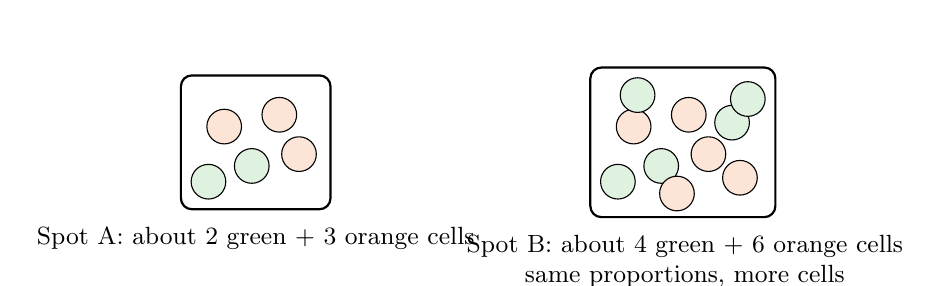
\begin{tikzpicture}[x=1cm,y=1cm, every node/.style={font=\small,align=center}]
  \foreach \x/\y/\c in {0/0/softgreen,0.55/0.2/softgreen,0.2/0.7/softorange,0.9/0.85/softorange,1.15/0.35/softorange}
    \draw[fill=\c, draw=black] (\x,\y) circle (0.22);
  \draw[thick, rounded corners] (-0.35,-0.35) rectangle (1.55,1.35);
  \node[below] at (0.6,-0.45) {Spot A: about 2 green + 3 orange cells};

  \begin{scope}[xshift=5.2cm]
  \foreach \x/\y/\c in {0/0/softgreen,0.55/0.2/softgreen,0.2/0.7/softorange,0.9/0.85/softorange,1.15/0.35/softorange,1.45/0.75/softgreen,0.75/-0.15/softorange,1.55/0.05/softorange,0.25/1.1/softgreen,1.65/1.05/softgreen}
    \draw[fill=\c, draw=black] (\x,\y) circle (0.22);
  \draw[thick, rounded corners] (-0.35,-0.45) rectangle (2.0,1.45);
  \node[below, align=center] at (0.85,-0.55) {Spot B: about 4 green + 6 orange cells\\same proportions, more cells};
  \end{scope}
\end{tikzpicture}
\caption{Two spots can have the same proportions but different absolute cell abundances. Cell2location tries to estimate abundance, not only percentages.}
\end{figure}

\section{The model as a generative story}

A \term{generative story} describes how data could be produced if we knew all the hidden quantities. Cell2location's story can be simplified as follows.

\begin{enumerate}
  \item For each spot $s$, choose hidden cell-type abundances $w_{s,1},\ldots,w_{s,F}$.
  \item Use reference signatures $g_{f,g}$ to predict how much each gene should appear from that mixture.
  \item Adjust for technology with $m_g$, background RNA with $s_{e,g}$, and spot sensitivity with $y_s$.
  \item This gives an expected count $\mu_{s,g}$ for every spot and gene.
  \item Draw the observed count $d_{s,g}$ from a negative binomial distribution centered around $\mu_{s,g}$.
\end{enumerate}

Bayesian inference reverses this. We already have the observed $d_{s,g}$. We want to infer the likely $w_{s,f}$ and other unknowns.

\begin{figure}[H]
\centering
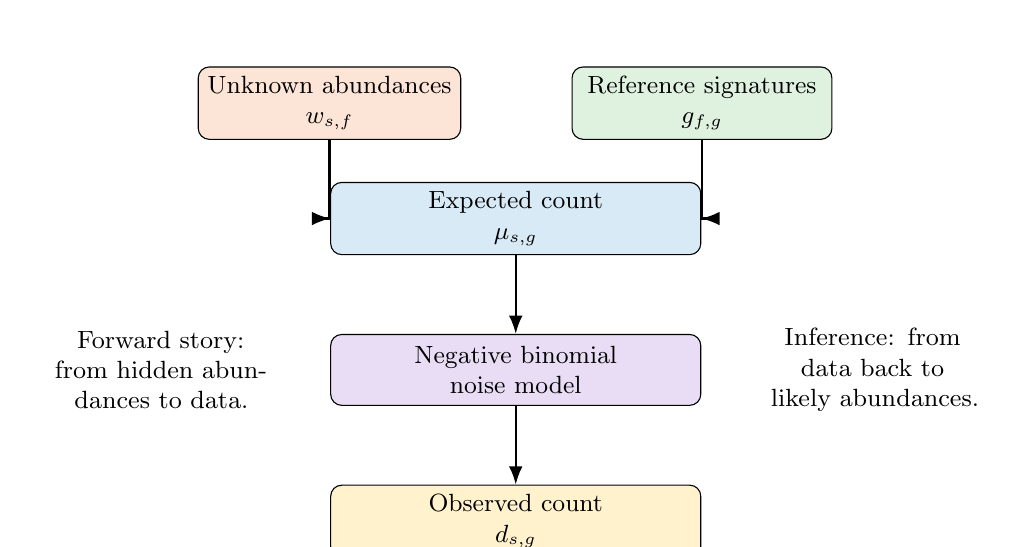
\begin{tikzpicture}[node distance=1.0cm, every node/.style={font=\small,align=center}, >=Latex]
  \node[draw, rounded corners, fill=softorange, minimum width=3.3cm, minimum height=0.9cm] (w) {Unknown abundances\\$w_{s,f}$};
  \node[draw, rounded corners, fill=softgreen, right=1.4cm of w, minimum width=3.3cm, minimum height=0.9cm] (sig) {Reference signatures\\$g_{f,g}$};
  \node[draw, rounded corners, fill=softblue, below=1.0cm of $(w)!0.5!(sig)$, minimum width=4.7cm, minimum height=0.9cm] (mu) {Expected count\\$\mu_{s,g}$};
  \node[draw, rounded corners, fill=softpurple, below=1.0cm of mu, minimum width=4.7cm, minimum height=0.9cm] (dist) {Negative binomial\\noise model};
  \node[draw, rounded corners, fill=lightyellow, below=1.0cm of dist, minimum width=4.7cm, minimum height=0.9cm] (d) {Observed count\\$d_{s,g}$};
  \draw[->, thick] (w) |- (mu);
  \draw[->, thick] (sig) |- (mu);
  \draw[->, thick] (mu) -- (dist);
  \draw[->, thick] (dist) -- (d);
  \node[align=center, left=0.5cm of dist, text width=3.1cm] {Forward story: from hidden abundances to data.};
  \node[align=center, right=0.5cm of dist, text width=3.1cm] {Inference: from data back to likely abundances.};
\end{tikzpicture}
\caption{The generative direction goes from hidden cell abundance to observed counts. Inference goes in the reverse direction.}
\end{figure}

\section{Where do priors enter?}

A prior is a probability model for an unknown before the current data are used. It is not random guessing. It is a way to include reasonable background information.

In cell2location, priors help with questions such as:

\begin{itemize}
  \item Are cell abundances allowed to be negative? No. Priors keep $w_{s,f}\ge 0$.
  \item Is it reasonable to estimate 400 cells in one Visium spot? Usually no. The expected cell abundance prior discourages unreasonable totals.
  \item Should neighboring or similar tissue locations have completely unrelated cell mixtures? Usually no. The hierarchical prior encourages sharing information.
  \item Should spot sensitivity $y_s$ vary wildly from spot to spot? Usually no, unless the data suggest strong technical gradients.
\end{itemize}

\begin{bigidea}
The likelihood asks, ``Which values explain the counts?'' The prior asks, ``Which values were reasonable before seeing these counts?'' The posterior balances both.
\end{bigidea}

\subsection{Priors do not erase data}

A prior is not a command. If the data strongly disagree with the prior, the posterior can move away from the prior. But if data are weak or ambiguous, the prior has more influence.

This is especially important for rare or fine-grained cell types. If a rare cell type has only a weak signal, the hierarchical prior can help by borrowing information from other spots that look similar.

\section{What are hyperparameters?}

A parameter is an unknown inside the model. A hyperparameter is a setting that controls a prior or model behavior.

\begin{center}
\begin{tabularx}{0.95\textwidth}{>{\bfseries}p{0.28\textwidth}X}
\toprule
Word & Meaning \\
\midrule
Parameter & A quantity the model estimates from the data, such as $w_{s,f}$ or $y_s$. \\
Prior & A probability distribution placed on an unknown parameter. \\
Hyperparameter & A knob that controls the prior. Often set by the user using outside knowledge. \\
Posterior & The updated distribution over parameters after seeing the data. \\
\bottomrule
\end{tabularx}
\end{center}

\subsection{Analogy: a teacher grading essays}

Suppose a teacher expects high-school essays to be around 500 words. This expectation is not the essay itself. It is a guideline.

\begin{itemize}
  \item The actual essay length is like a \term{parameter}.
  \item The belief that essays are usually around 500 words is like a \term{prior}.
  \item The number 500 is like a \term{hyperparameter}.
\end{itemize}

In cell2location, $\hat N$ is like saying, ``I expect about this many cells per spot.'' The model can adjust based on data, but this expectation guides absolute cell abundance estimates.

\section{The two user-adjusted hyperparameters on page 12}

Page 12 highlights two parameters that users should adjust based on the dataset.

\begin{mathbox}
\[
\boxed{\hat N = \text{expected cell abundance per spot}}
\]
\[
\boxed{\alpha^y = \text{regularization strength for spot sensitivity } y_s}
\]
\end{mathbox}

\subsection{Hyperparameter 1: expected cell abundance per spot}

$\hat N$ tells the model roughly how many cells are expected in a spot. It can be estimated from histology images by counting nuclei in 10-20 locations and taking the average.

\begin{bigidea}
$\hat N$ is especially important for estimating \emph{absolute} cell abundance. If you want the model to say ``about 8 cells'' rather than only ``about 40 percent T cells,'' you need a reasonable idea of how many cells a spot usually contains.
\end{bigidea}

\subsubsection{Example}

If a tissue image shows about 8 nuclei per spot, you might set $\hat N\approx 8$.

If you set $\hat N$ much too high, the model may be nudged toward too many cells per spot. If you set it much too low, it may be nudged toward too few. The paper notes the model is robust to a range of similar values, but good choices help.

\begin{figure}[H]
\centering
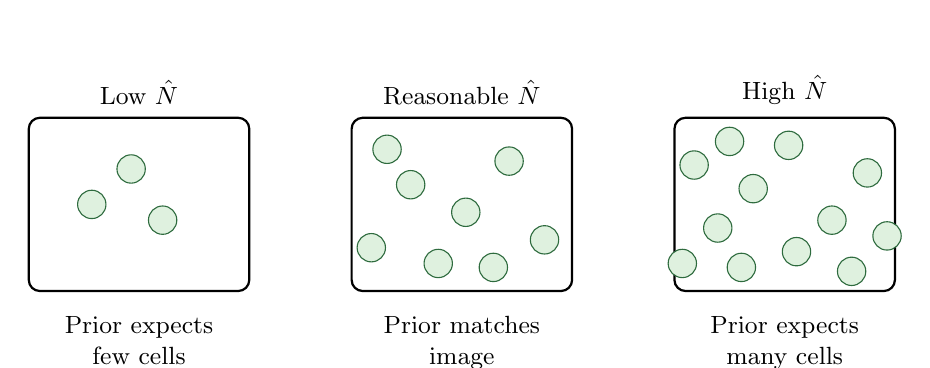
\begin{tikzpicture}[x=1cm,y=1cm,every node/.style={font=\small,align=center}]
  \foreach \i/\n in {0/Low $\hat N$,1/Reasonable $\hat N$,2/High $\hat N$}{
    \begin{scope}[xshift=4.1*\i cm]
      \draw[rounded corners, thick] (0,0) rectangle (2.8,2.2);
      \node[above] at (1.4,2.25) {\n};
    \end{scope}
  }
  \foreach \p in {(0.8,1.1),(1.7,0.9),(1.3,1.55)}
    \draw[fill=softgreen, draw=darkgreen] \p circle (0.18);
  \foreach \p in {(4.35,0.55),(4.85,1.35),(5.55,1.0),(6.1,1.65),(6.55,0.65),(5.2,0.35),(4.55,1.8),(5.9,0.3)}
    \draw[fill=softgreen, draw=darkgreen] \p circle (0.18);
  \foreach \p in {(8.3,0.35),(8.75,0.8),(9.2,1.3),(9.75,0.5),(10.2,0.9),(10.65,1.5),(8.45,1.6),(9.05,0.3),(9.65,1.85),(10.45,0.25),(8.9,1.9),(10.9,0.7)}
    \draw[fill=softgreen, draw=darkgreen] \p circle (0.18);
  \node[align=center, below] at (1.4,-0.2) {Prior expects\\few cells};
  \node[align=center, below] at (5.5,-0.2) {Prior matches\\image};
  \node[align=center, below] at (9.6,-0.2) {Prior expects\\many cells};
\end{tikzpicture}
\caption{$\hat N$ is a prior expectation about total cells per spot. It should be estimated from the tissue image when possible.}
\end{figure}

\subsection{Hyperparameter 2: regularization of spot sensitivity}

$\alpha^y$ controls the prior on $y_s$, the spot-level RNA detection sensitivity.

Page 12 says $\alpha^y$ is the shape parameter of a gamma prior over $y_s$. For intuition, you do not need the full gamma math. Think of $\alpha^y$ as controlling how tightly the model expects $y_s$ to stay near the experiment's average sensitivity.

\begin{center}
\begin{tabularx}{0.95\textwidth}{>{\bfseries}p{0.24\textwidth}X}
\toprule
Choice of $\alpha^y$ & Intuition \\
\midrule
Large $\alpha^y$, such as 200 & Strong regularization. Spot sensitivities $y_s$ are expected to be close to the batch average. Use when RNA detection is fairly uniform across spots. \\
Smaller $\alpha^y$, such as 20 & Weaker regularization. Spot sensitivities $y_s$ are allowed to vary more. Use when there are strong spatial gradients or uneven RNA detection. \\
\bottomrule
\end{tabularx}
\end{center}

\begin{figure}[H]
\centering
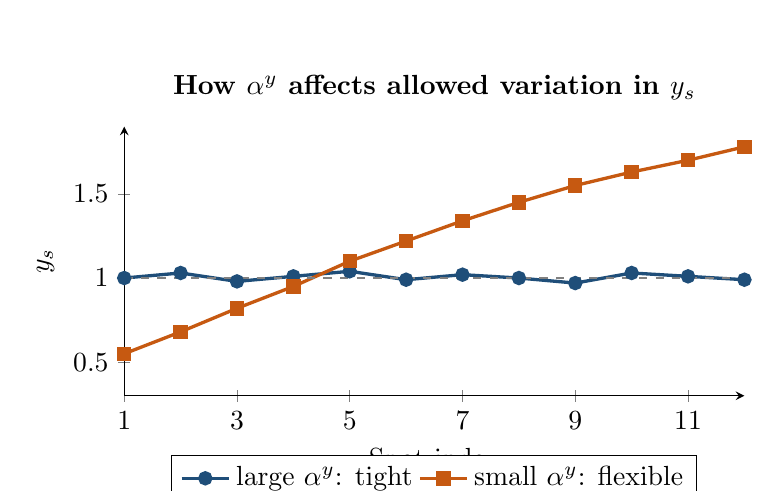
\begin{tikzpicture}
\begin{axis}[
  width=0.78\textwidth,
  height=5cm,
  xlabel={Spot index},
  ylabel={$y_s$},
  ymin=0.3,ymax=1.9,
  xmin=1,xmax=12,
  xtick={1,3,5,7,9,11},
  ytick={0.5,1.0,1.5},
  legend style={at={(0.5,-0.22)},anchor=north,legend columns=2},
  axis lines=left,
  title={How $\alpha^y$ affects allowed variation in $y_s$},
  title style={font=\bfseries}
]
\addplot[deepblue, very thick, mark=*] coordinates {(1,1.00)(2,1.03)(3,0.98)(4,1.01)(5,1.04)(6,0.99)(7,1.02)(8,1.00)(9,0.97)(10,1.03)(11,1.01)(12,0.99)};
\addlegendentry{large $\alpha^y$: tight}
\addplot[darkorange, very thick, mark=square*] coordinates {(1,0.55)(2,0.68)(3,0.82)(4,0.95)(5,1.10)(6,1.22)(7,1.34)(8,1.45)(9,1.55)(10,1.63)(11,1.70)(12,1.78)};
\addlegendentry{small $\alpha^y$: flexible}
\draw[black!50, dashed] (axis cs:1,1) -- (axis cs:12,1);
\end{axis}
\end{tikzpicture}
\caption{Schematic only. A large $\alpha^y$ keeps spot sensitivity near the average. A smaller $\alpha^y$ allows stronger spot-to-spot sensitivity differences.}
\end{figure}

\begin{warningbox}
Regularization means ``do not let this parameter wiggle too much unless the data really need it.'' Large $\alpha^y$ means stronger regularization for $y_s$.
\end{warningbox}

\section{The hierarchical part: borrowing strength across locations}

Page 12 says the cell type abundance estimates $w_{s,f}$ are not independent across locations. Why? Because tissues are organized into regions. Nearby or similar spots often have similar mixtures of cell types.

For example, in brain tissue, one region may mostly contain one group of neuron subtypes, while another region contains a different group. In a lymph node, some regions contain B-cell zones and others contain T-cell zones.

\begin{bigidea}
``Borrowing statistical strength'' means using patterns learned from many related spots to help estimate a difficult spot. This is useful when the signal for a rare or fine-grained cell type is weak at one location.
\end{bigidea}

\subsection{A school analogy}

Suppose one student misses part of a quiz, but you know they studied with a group and their answers on other questions are similar to that group. You would not copy the group's answers blindly, but the group gives useful context.

Similarly, a spot with noisy data can be helped by other spots that appear to belong to the same tissue zone.

\begin{figure}[H]
\centering
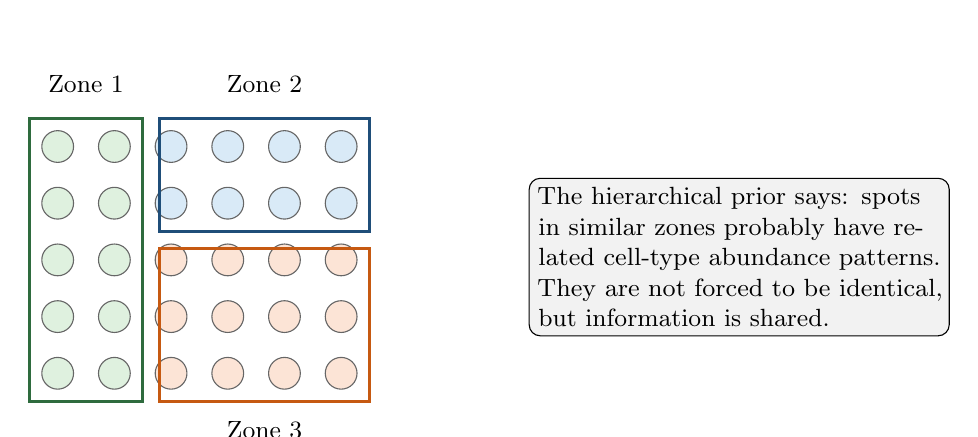
\begin{tikzpicture}[x=0.72cm,y=0.72cm,every node/.style={font=\small,align=center}]
  \foreach \x in {0,...,5}{
    \foreach \y in {0,...,4}{
      \pgfmathtruncatemacro{\region}{ifthenelse(\x<2,0,ifthenelse(\y>2,1,2))}
      \ifnum\region=0
        \def\fillcol{softgreen}
      \else\ifnum\region=1
        \def\fillcol{softblue}
      \else
        \def\fillcol{softorange}
      \fi\fi
      \draw[fill=\fillcol, draw=black!60] (\x,\y) circle (0.28);
    }
  }
  \draw[very thick, darkgreen] (-0.5,-0.5) rectangle (1.5,4.5);
  \draw[very thick, deepblue] (1.8,2.5) rectangle (5.5,4.5);
  \draw[very thick, darkorange] (1.8,-0.5) rectangle (5.5,2.2);
  \node[align=center] at (0.5,5.1) {Zone 1};
  \node[align=center] at (3.65,5.1) {Zone 2};
  \node[align=center] at (3.65,-1.0) {Zone 3};

  \node[draw, rounded corners, fill=softgray, right=2.0cm of current bounding box.east, text width=5.1cm, align=left] (text) {The hierarchical prior says: spots in similar zones probably have related cell-type abundance patterns. They are not forced to be identical, but information is shared.};
\end{tikzpicture}
\caption{A schematic tissue grid. Spots in the same zone often share cell compositions. The hierarchical model uses that fact.}
\end{figure}

\subsection{What is the ``factorization'' idea?}

Page 12 says $w_{s,f}$ is modeled with a hierarchical decomposition prior, assuming $R$ groups of cell types that partly share common abundance profiles. Unless stated otherwise, $R=50$ in the paper.

A simplified way to imagine this is:

\[
\text{cell abundance at spot }s
\approx
\text{combination of several tissue-zone patterns}.
\]

This does \emph{not} mean there are exactly 50 biological tissue zones. Instead, $R=50$ is a flexible model setting that gives the model enough reusable patterns to represent many spatial structures.

\section{Reference cell-type signatures}

Cell2location needs reference signatures $g_{f,g}$. These usually come from single-cell or single-nucleus RNA-seq data.

\begin{mathbox}
\[
g_{f,g} = \text{expected expression of gene } g \text{ in cell type } f.
\]
\end{mathbox}

\subsection{Why signatures matter}

If the reference says T cells express Gene A and B cells express Gene B, then a spot with lots of Gene A is evidence for T cells, and a spot with lots of Gene B is evidence for B cells.

But the reference must be reasonably comprehensive. If a cell type is missing from the reference, the model may try to explain its RNA using the closest available cell types.

\begin{assumptionbox}
The model assumes the reference signatures are good enough to explain the spatial data. They do not have to be perfect, but important missing cell types or badly mismatched signatures can hurt the results.
\end{assumptionbox}

\subsection{Why use negative binomial regression to estimate signatures?}

Page 12 says the signature matrix is often estimated using a negative binomial regression model. The reason is that single-cell data also have count noise and batch effects. A model-based signature estimate can combine data across batches and technologies more robustly than simply averaging counts.

However, the page also notes that if batch effects are small, a simpler per-cluster average can be enough. For some non-UMI technologies, the negative binomial count model may not be appropriate, so a simpler method can be recommended.

\section{The full model in plain English}

Here is the page-12 model translated sentence by sentence.

\begin{longtable}{p{0.32\textwidth}p{0.60\textwidth}}
\toprule
Mathematical phrase & Plain-English translation \\
\midrule
$d_{s,g}$ & The count we observed for gene $g$ in spot $s$. \\
$d_{s,g}\sim \NB(\mu_{s,g},\alpha_{e,g})$ & The observed count is noisy. It tends to be near $\mu_{s,g}$, but can vary. $\alpha_{e,g}$ controls extra count variability. \\
$\mu_{s,g}$ & The expected count before random noise is added. \\
$\sum_f w_{s,f}g_{f,g}$ & Add up contributions from every cell type. For each cell type: abundance in the spot times that cell type's expression of the gene. \\
$m_g$ & Adjusts gene $g$ for technology-specific sensitivity. \\
$s_{e,g}$ & Adds possible background or contaminating RNA for gene $g$ in experiment $e$. \\
$y_s$ & Adjusts for how much RNA was detected at spot $s$ overall. \\
$w_{s,f}$ & The main answer: abundance of cell type $f$ in spot $s$. \\
Hierarchical prior on $w_{s,f}$ & Spots in similar tissue regions share information, helping noisy or rare-cell estimates. \\
Variational inference & A fast approximate way to find the posterior distributions of the unknowns. \\
\bottomrule
\end{longtable}

\section{How Bayesian inference works here, step by step}

\subsection{Step A: propose possible cell mixtures}

For a spot, the model considers many possible values of $w_{s,f}$. For example:

\begin{center}
\begin{tabular}{lccc}
\toprule
Candidate & T cells & B cells & Astrocytes \\
\midrule
1 & 0 & 5 & 0 \\
2 & 2 & 3 & 0 \\
3 & 1 & 1 & 4 \\
4 & 5 & 0 & 0 \\
\bottomrule
\end{tabular}
\end{center}

Real cell2location does not literally list only four candidates. It uses continuous probability distributions and optimization. But this mental picture is useful.

\subsection{Step B: compute predicted gene counts}

For each candidate, use the reference signatures and technical corrections to compute $\mu_{s,g}$ for every gene.

\subsection{Step C: compare predictions to observed counts}

The negative binomial likelihood gives a score: how likely are the observed counts if this candidate mixture were true?

\subsection{Step D: combine with priors}

Candidates that have impossible or unreasonable abundances are discouraged by priors. For example, negative cell abundance is impossible, and a total of 100 cells in a spot with $\hat N=8$ is unlikely unless the data strongly demand it.

\subsection{Step E: output posterior estimates}

The final output is a posterior distribution for the cell abundances. In practice, software often reports summary values such as posterior mean abundance.

\begin{figure}[H]
\centering
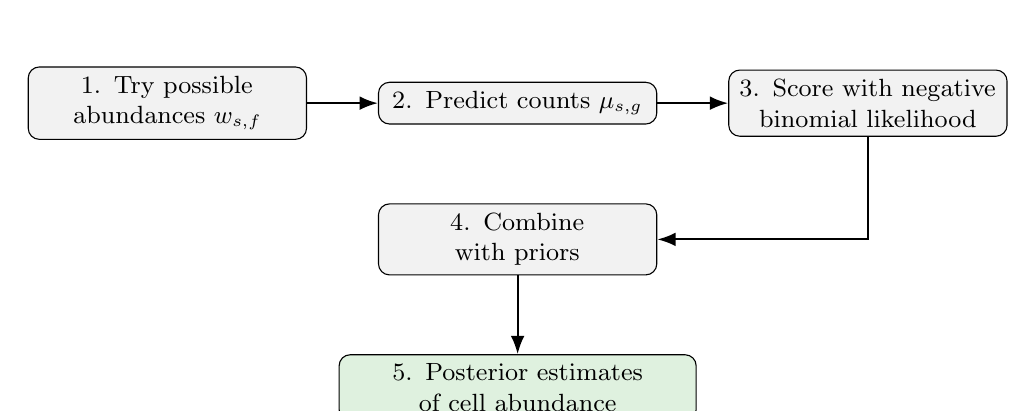
\begin{tikzpicture}[node distance=0.85cm, every node/.style={font=\small,align=center}, >=Latex]
  \node[draw, rounded corners, fill=softgray, text width=3.3cm, align=center] (p1) {1. Try possible abundances $w_{s,f}$};
  \node[draw, rounded corners, fill=softgray, right=0.9cm of p1, text width=3.3cm, align=center] (p2) {2. Predict counts $\mu_{s,g}$};
  \node[draw, rounded corners, fill=softgray, right=0.9cm of p2, text width=3.3cm, align=center] (p3) {3. Score with negative binomial likelihood};
  \node[draw, rounded corners, fill=softgray, below=1.0cm of p2, text width=3.3cm, align=center] (p4) {4. Combine with priors};
  \node[draw, rounded corners, fill=softgreen, below=1.0cm of p4, text width=4.3cm, align=center] (p5) {5. Posterior estimates of cell abundance};
  \draw[->, thick] (p1) -- (p2);
  \draw[->, thick] (p2) -- (p3);
  \draw[->, thick] (p3) |- (p4);
  \draw[->, thick] (p4) -- (p5);
\end{tikzpicture}
\caption{A beginner-level view of inference. The real algorithm is more advanced, but it follows this logic.}
\end{figure}

\section{Variational inference: why the paper says ``approximate''}

A full Bayesian posterior can be very complicated. Cell2location has thousands or millions of unknowns: abundances for many spots and cell types, gene effects, batch effects, sensitivities, and noise parameters.

Instead of calculating the exact posterior, the software uses \term{approximate variational inference}. Here is the idea:

\begin{itemize}
  \item Pick a flexible but manageable family of probability distributions.
  \item Adjust that distribution until it is close to the true posterior.
  \item Use optimization, often with GPU acceleration, to do this fast.
\end{itemize}

\begin{bigidea}
Variational inference is like drawing a simpler map of a complicated city. The map is not the city itself, but if it is accurate enough, it helps you navigate quickly.
\end{bigidea}

\section{Assumptions made by the model}

Every model has assumptions. Good science means knowing them.

\begin{assumptionbox}
\term{Assumption 1: additive mixtures.} The gene expression in a spot is approximately a sum of contributions from cell types. This is the main mixture assumption.
\end{assumptionbox}

\begin{assumptionbox}
\term{Assumption 2: reference signatures are useful.} The signatures $g_{f,g}$ represent the cell types in the tissue well enough. Missing or incorrect cell types can mislead the model.
\end{assumptionbox}

\begin{assumptionbox}
\term{Assumption 3: negative binomial count noise.} Given $\mu_{s,g}$ and $\alpha_{e,g}$, the observed counts behave like negative binomial count data. This is common for RNA counts but is still a modeling choice.
\end{assumptionbox}

\begin{assumptionbox}
\term{Assumption 4: technical effects can be summarized by model terms.} Gene sensitivity $m_g$, background shift $s_{e,g}$, and spot sensitivity $y_s$ are assumed to capture important technical variation.
\end{assumptionbox}

\begin{assumptionbox}
\term{Assumption 5: locations can share information.} The hierarchical prior assumes tissue organization creates repeated spatial patterns, so spots are not estimated in total isolation.
\end{assumptionbox}

\section{Common misunderstandings}

\subsection{Misunderstanding 1: ``The model knows the true number of cells''}

No. It estimates abundance from noisy data. The output is an informed estimate, not direct observation of every cell.

\subsection{Misunderstanding 2: ``A hyperparameter is another cell abundance''}

No. A hyperparameter is a setting that shapes a prior. $\hat N$ is not the number of cells in one specific spot; it is a prior expectation for a typical spot.

\subsection{Misunderstanding 3: ``The prior is cheating''}

No. Priors are part of Bayesian modeling. They make assumptions explicit. For example, knowing from an image that a spot usually has about 8 cells is useful information, not cheating.

\subsection{Misunderstanding 4: ``If the model has many terms, it must be arbitrary''}

Not necessarily. Each term has a job:

\begin{center}
\begin{tabular}{ll}
\toprule
Term & Job \\
\midrule
$w_{s,f}$ & biology: cell abundance \\
$g_{f,g}$ & biology/reference: cell-type expression pattern \\
$m_g$ & technology-specific gene scaling \\
$s_{e,g}$ & background RNA \\
$y_s$ & spot sensitivity \\
$\alpha_{e,g}$ & extra count noise \\
\bottomrule
\end{tabular}
\end{center}

\subsection{Misunderstanding 5: ``A high count for one gene proves one cell type is present''}

Not always. One gene can be shared by multiple cell types, and counts are noisy. Cell2location uses many genes together, which is much stronger than relying on one marker gene.

\section{A complete summary diagram}

\begin{figure}[H]
\centering
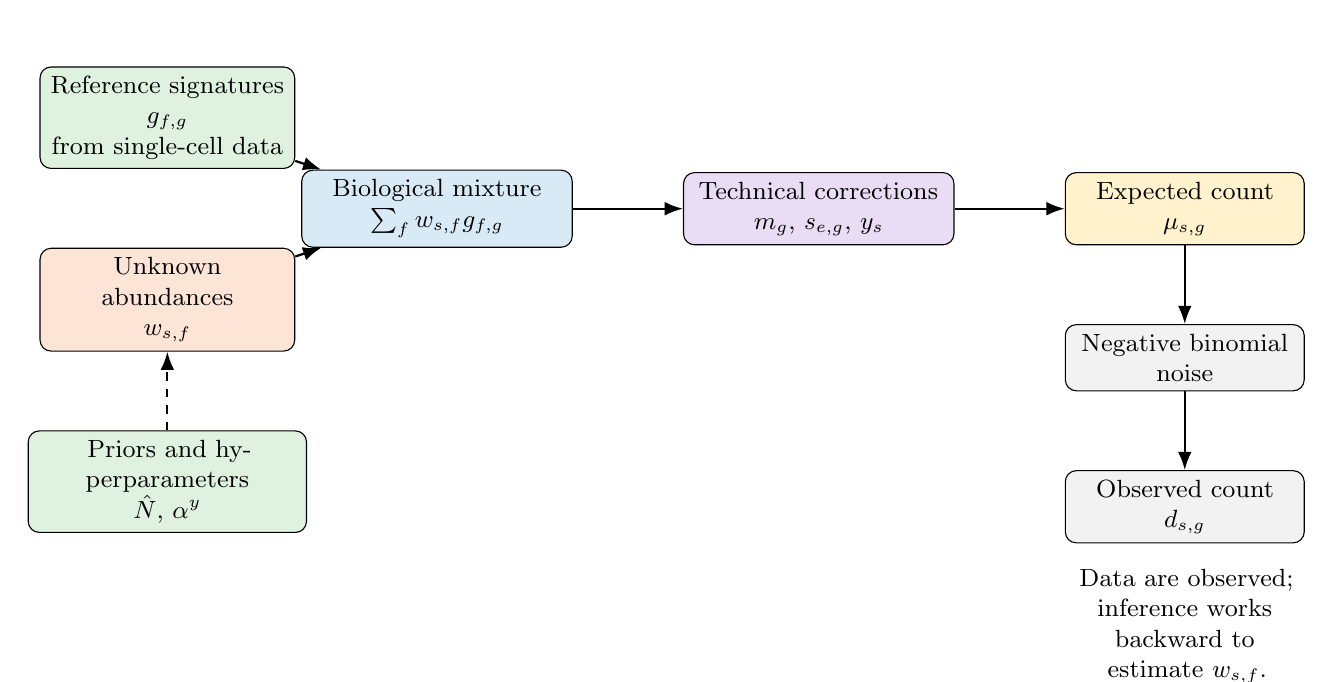
\begin{tikzpicture}[every node/.style={font=\small,align=center}, >=Latex]
  \node[draw, rounded corners, fill=softgreen, text width=3.0cm, align=center] (ref) {Reference signatures\\$g_{f,g}$\\from single-cell data};
  \node[draw, rounded corners, fill=softorange, below=1.0cm of ref, text width=3.0cm, align=center] (w) {Unknown abundances\\$w_{s,f}$};
  \node[draw, rounded corners, fill=softblue, right=1.7cm of $(ref)!0.5!(w)$, text width=3.2cm, align=center] (mix) {Biological mixture\\$\sum_f w_{s,f}g_{f,g}$};
  \node[draw, rounded corners, fill=softpurple, right=1.4cm of mix, text width=3.2cm, align=center] (tech) {Technical corrections\\$m_g$, $s_{e,g}$, $y_s$};
  \node[draw, rounded corners, fill=lightyellow, right=1.4cm of tech, text width=2.8cm, align=center] (mu) {Expected count\\$\mu_{s,g}$};
  \node[draw, rounded corners, fill=softgray, below=1.0cm of mu, text width=2.8cm, align=center] (nb) {Negative binomial\\noise};
  \node[draw, rounded corners, fill=softgray, below=1.0cm of nb, text width=2.8cm, align=center] (d) {Observed count\\$d_{s,g}$};
  \node[draw, rounded corners, fill=softgreen, below=1.0cm of w, text width=3.3cm, align=center] (prior) {Priors and hyperparameters\\$\hat N$, $\alpha^y$};
  \draw[->, thick] (ref) -- (mix);
  \draw[->, thick] (w) -- (mix);
  \draw[->, thick] (mix) -- (tech);
  \draw[->, thick] (tech) -- (mu);
  \draw[->, thick] (mu) -- (nb);
  \draw[->, thick] (nb) -- (d);
  \draw[->, thick, dashed] (prior) -- (w);
  \node[align=center, text width=3.0cm, below=0.2cm of d] {Data are observed; inference works backward to estimate $w_{s,f}$.};
\end{tikzpicture}
\caption{The cell2location model in one picture.}
\end{figure}

\section{How to read the original page-12 equation}

When you see this equation:

\[
\mu_{s,g}=\left(m_g\sum_f w_{s,f}g_{f,g}+s_{e,g}\right)y_s,
\]

read it slowly from the inside outward:

\begin{enumerate}
  \item $g_{f,g}$: cell type $f$'s usual expression of gene $g$.
  \item $w_{s,f}g_{f,g}$: contribution of cell type $f$ to gene $g$ in spot $s$.
  \item $\sum_f w_{s,f}g_{f,g}$: total biological contribution from all cell types.
  \item $m_g(\cdots)$: adjust gene $g$ for technology sensitivity.
  \item $+s_{e,g}$: add background RNA for gene $g$ in experiment $e$.
  \item $\times y_s$: adjust the whole spot for RNA-capture sensitivity.
  \item Result $\mu_{s,g}$: expected count of gene $g$ in spot $s$.
  \item Then $d_{s,g}\sim \NB(\mu_{s,g},\alpha_{e,g})$: observed counts are noisy around that expectation.
\end{enumerate}

\begin{checkpoint}
Try explaining this sentence out loud: ``The observed count is noisy, so the model first predicts an expected count from a mixture of cell-type signatures, then uses a negative binomial distribution to describe the random count we observe.'' If that sentence makes sense, you understand the main idea.
\end{checkpoint}

\section{Mini practice questions}

\begin{enumerate}
  \item If a spot has high counts for genes that are usually high in B cells, what should happen to $w_{s,B}$?
  \item If all genes in a spot are lower than expected, but the pattern across genes looks similar, which term might explain this: $w_{s,f}$, $m_g$, $s_{e,g}$, or $y_s$?
  \item If one gene is too high in every spot of one experiment, which term might help explain that?
  \item Why is $\hat N$ important for absolute abundance?
  \item Why might a hierarchical prior help with a rare cell type?
\end{enumerate}

\subsection*{Answers}

\begin{enumerate}
  \item $w_{s,B}$ should become larger, if the pattern fits B cells better than other cell types.
  \item $y_s$, because it changes the overall sensitivity of the spot.
  \item $s_{e,g}$ or $m_g$, because those are gene- and experiment/technology-related terms.
  \item Because it tells the model roughly how many cells are expected per spot, helping convert proportions into absolute cell counts.
  \item Rare cell types have weak signals. Sharing information across similar spots can make the estimate more stable.
\end{enumerate}

\section{One-page cheat sheet}

\begin{tcolorbox}[colback=softblue,colframe=deepblue,title=Cell2location page-12 model cheat sheet,fonttitle=\bfseries,breakable]
\textbf{Goal.} Estimate $w_{s,f}$, the abundance of cell type $f$ at spot $s$.

\textbf{Observed data.} $d_{s,g}$ = RNA count for gene $g$ at spot $s$.

\textbf{Reference input.} $g_{f,g}$ = typical expression of gene $g$ in cell type $f$.

\textbf{Expected count.}
\[
\mu_{s,g}=\left(m_g\sum_f w_{s,f}g_{f,g}+s_{e,g}\right)y_s.
\]

\textbf{Count noise.}
\[
d_{s,g}\sim \NB(\mu_{s,g},\alpha_{e,g}).
\]

\textbf{Technical terms.}
\begin{itemize}
  \item $m_g$: gene/technology sensitivity.
  \item $s_{e,g}$: background or contaminating RNA.
  \item $y_s$: spot-level RNA detection sensitivity.
  \item $\alpha_{e,g}$: extra count variability.
\end{itemize}

\textbf{Priors and hyperparameters.}
\begin{itemize}
  \item $\hat N$: expected cells per spot. Estimate from tissue images when possible.
  \item $\alpha^y$: how strongly $y_s$ is kept near the batch average. Larger means tighter; smaller means more flexible.
\end{itemize}

\textbf{Main assumptions.}
Spots are mixtures of cell-type signatures; counts are noisy negative-binomial counts; reference signatures are useful; technical variation can be represented by the model terms; related locations can share information.
\end{tcolorbox}

\section*{Source note}
\addcontentsline{toc}{section}{Source note}
This tutorial explains the Bayesian model described in the Methods section, especially page 12, of Kleshchevnikov et al., \emph{Cell2location maps fine-grained cell types in spatial transcriptomics}, \emph{Nature Biotechnology} 40, 661--671 (2022). The tutorial is written as an educational paraphrase with simplified examples and diagrams.

\end{document}
